% !TeX root = ../main.tex
\documentclass[./../main.tex]{subfiles}

\begin{document}

Phần này mô tả sản phẩm cuối sau quá trình phát triển của em, bao gồm
hình ảnh của giao diện người dùng thuộc phần client. Phần giao diện
người dùng sẽ được bạn Phạm Thị Dân mô tả kỹ hơn ở một báo cáo khác.

\subsubsection{Màn hình đăng nhập}

% 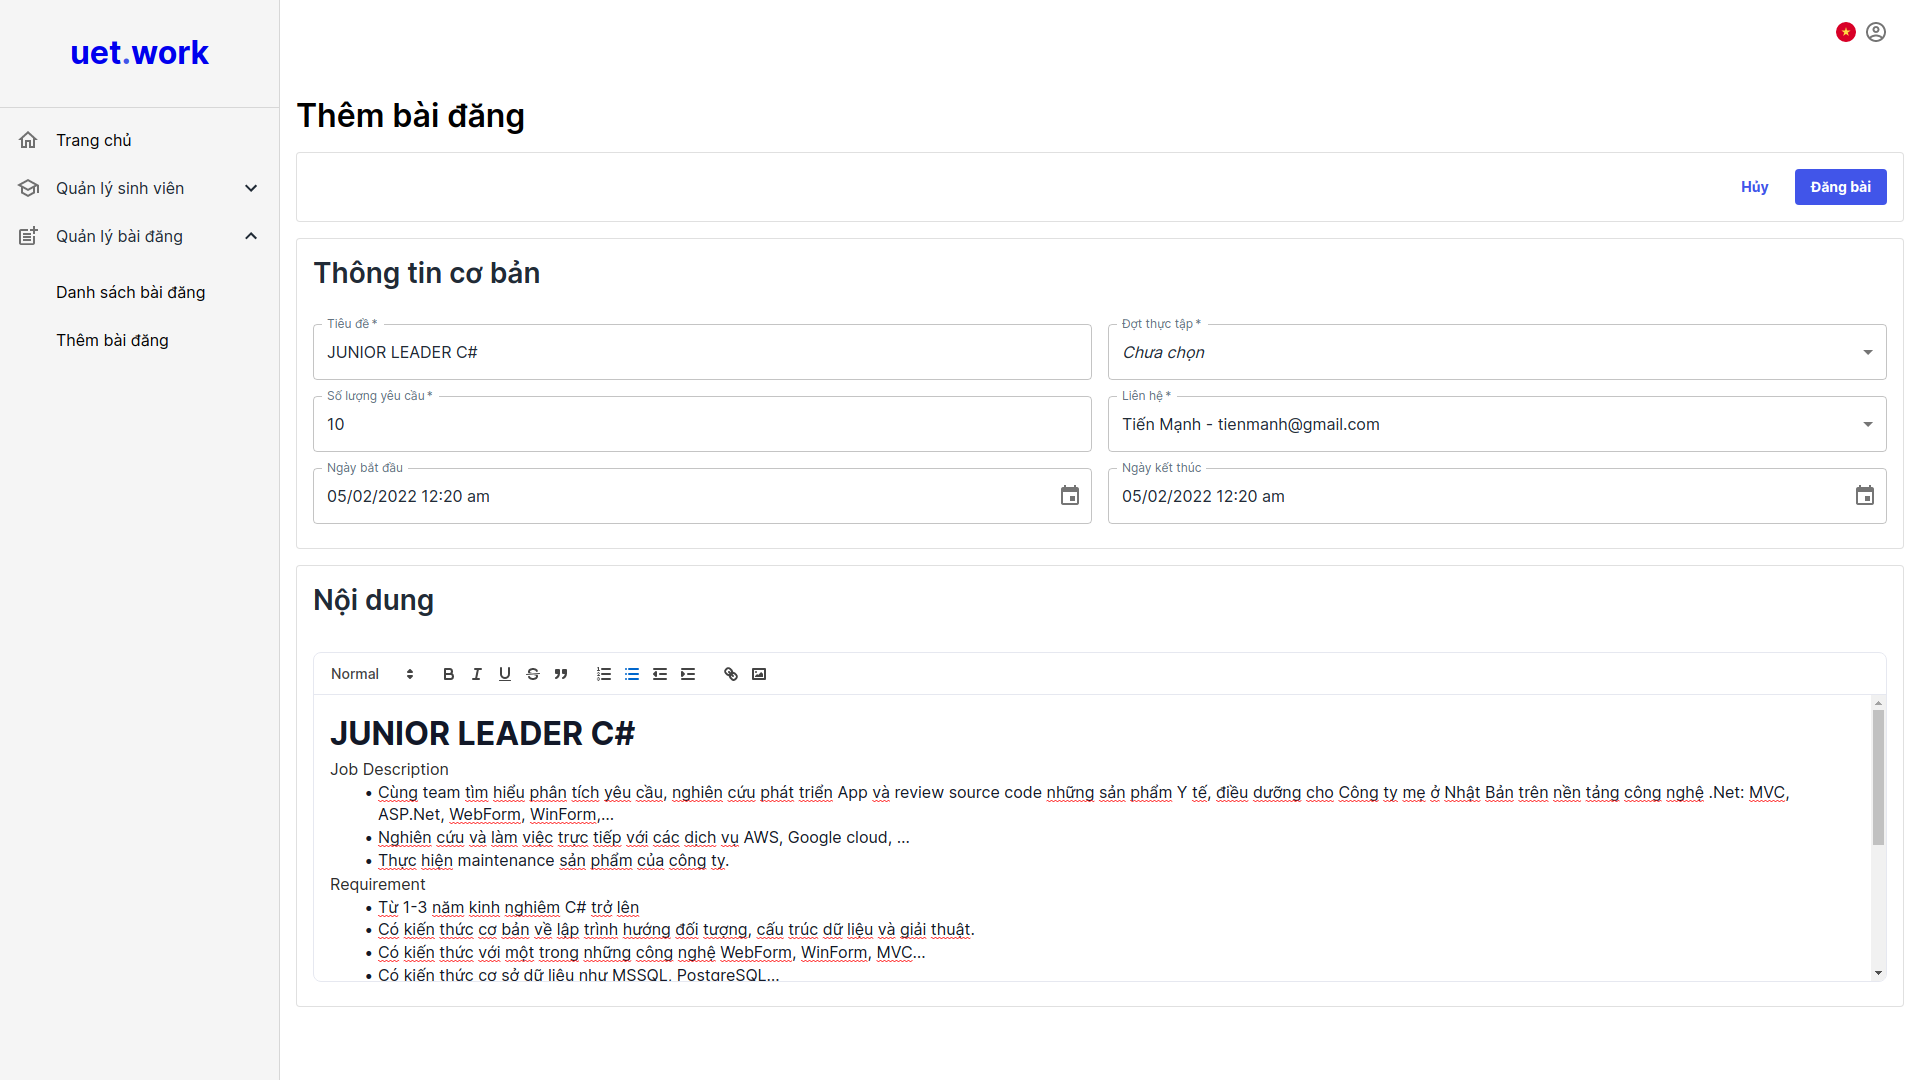
\includegraphics[width=6.5in,height=4.31944in]{vertopal_840b8d8141ff4800a3d2d1a844259cf5/media/image18.png}

Người dùng điền thông tin tài khoản và mật khẩu, hoặc lựa chọn đăng nhập
bằng Google để đăng nhập vào hệ thống. Hệ thống sẽ dựa vào vai trò của
người dùng là sinh viên, giảng viên, đối tác hay quản trị viên để điều
hướng người dùng tới trang phù hợp.

\subsubsection{Màn hình của Sinh viên}

Nếu người dùng là \textbf{sinh viên}, hệ thống sẽ hiển thị màn hình
trang chủ của sinh viên. Tại đây, sinh viên có thể đăng ký thực tập tại
một công ty hoặc đọc các bài đăng tuyển dụng và đăng ký phỏng vấn. Ngoài
ra, tại trang \emph{Thông tin thực tập} và \emph{Trang thông tin cá
nhân}, người dùng có thể xem và chỉnh sửa các thông tin liên quan.

\subsubsection{Màn hình của Giảng viên}

% 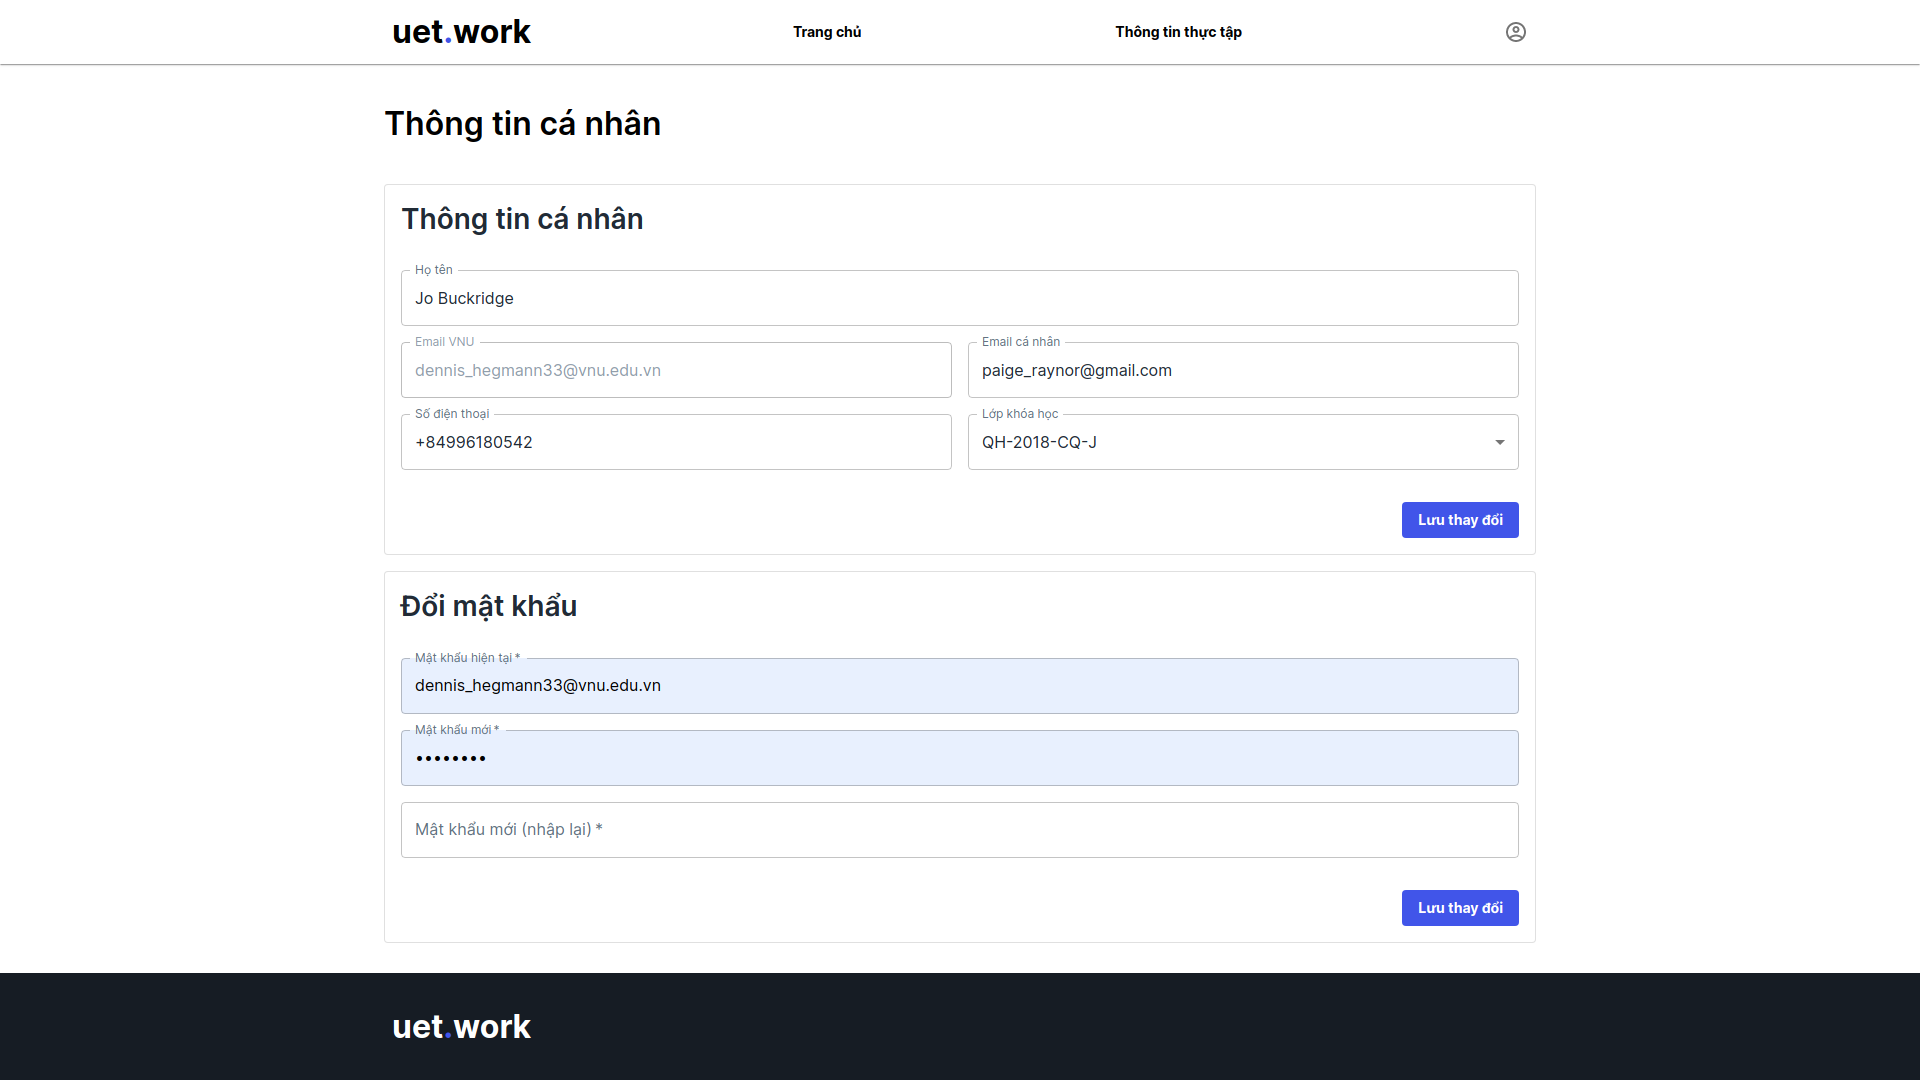
\includegraphics[width=6.5in,height=3.72222in]{vertopal_840b8d8141ff4800a3d2d1a844259cf5/media/image16.png}

Nếu người dùng là \textbf{giảng viên}, hệ thống sẽ hiển thị màn hình
trang chủ của giảng viên. Tại trang \emph{Sinh viên đang hướng dẫn},
giảng viên có thể xem, tìm kiếm, lọc ra danh sách các sinh viên đã nộp
báo cáo hay chưa, đã được chấm điểm hay chưa, và có thể thêm điểm cho
sinh viên.

\subsubsection{Màn hình của Đối tác}

% 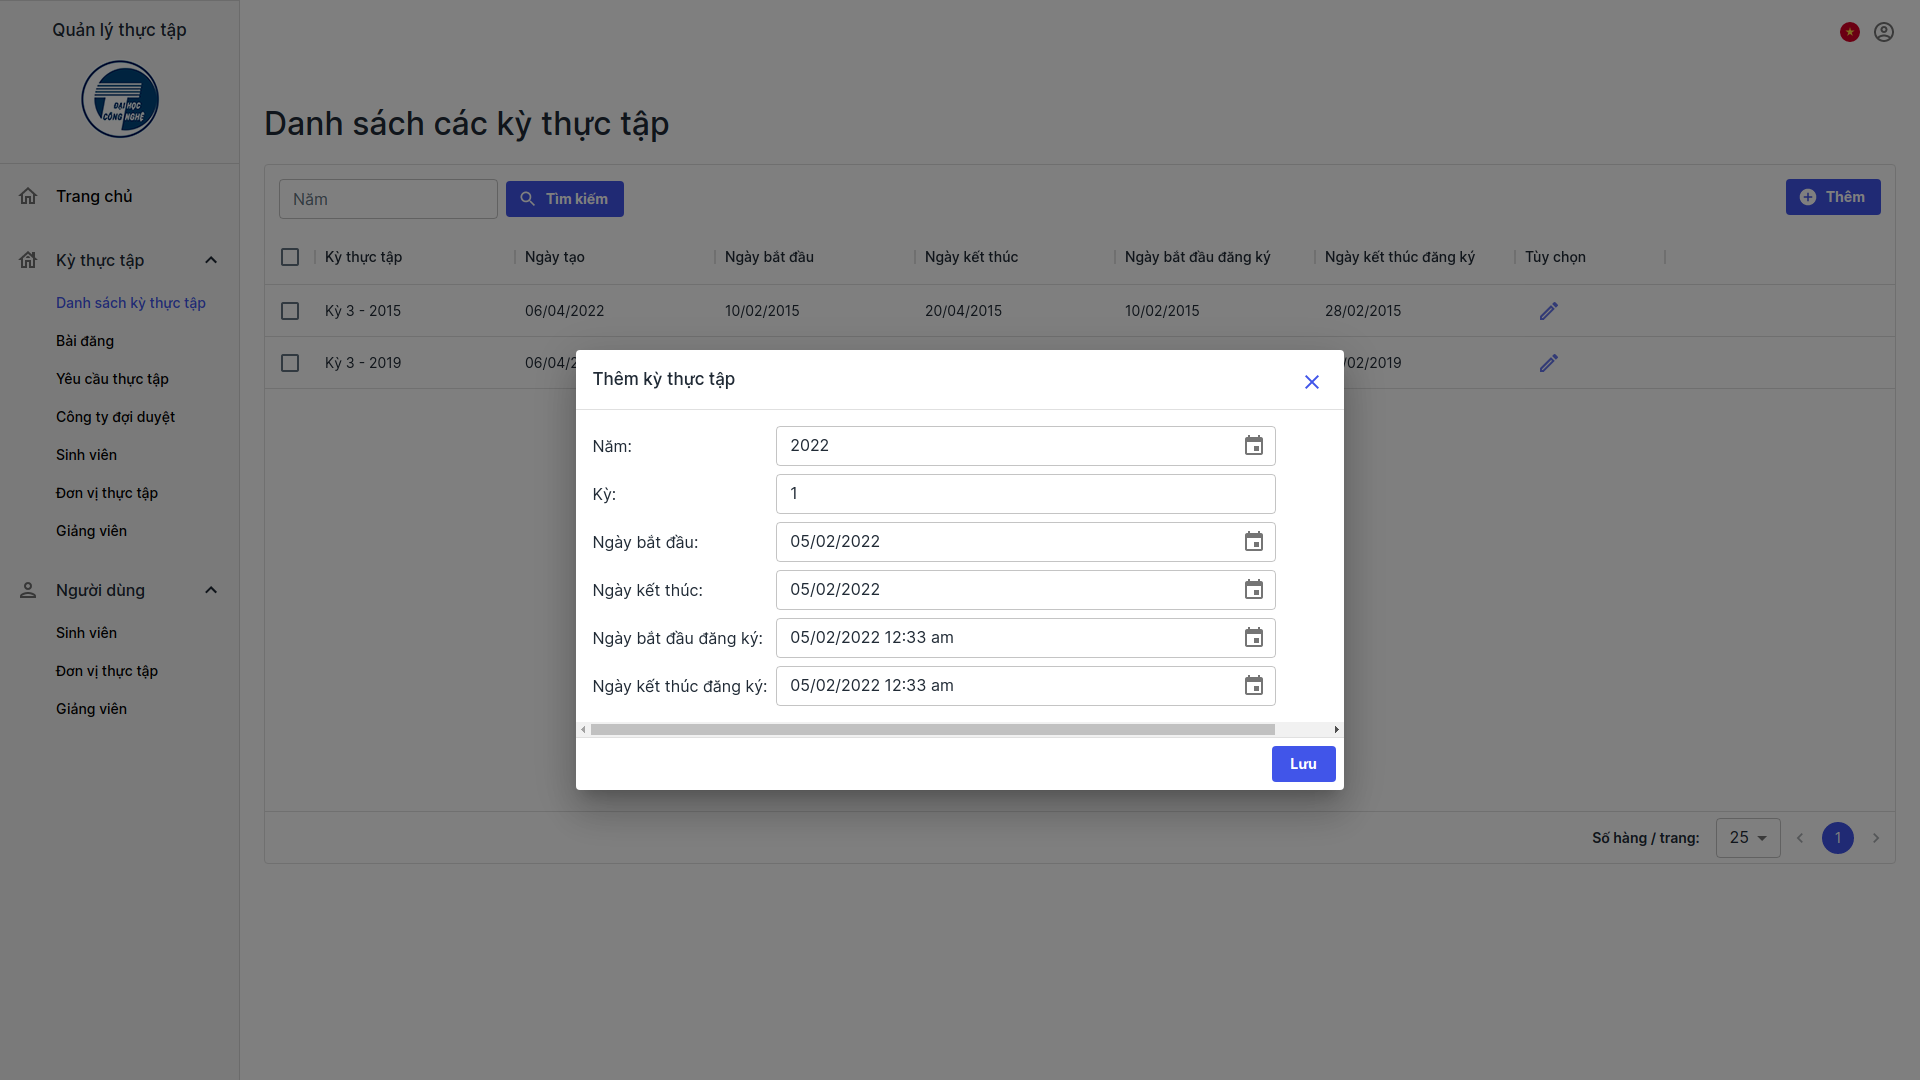
\includegraphics[width=6.5in,height=3.70833in]{vertopal_840b8d8141ff4800a3d2d1a844259cf5/media/image19.png}

Nếu người dùng là \textbf{đối tác}, hệ thống sẽ hiển thị màn hình trang
chủ của đối tác. Tại trang \emph{Sinh viên đang thực tập} và \emph{Yêu
cầu đăng ký thực tập,} đối tác có thể xem, lọc, tìm kiếm danh sách sinh
viên, chấp nhận / từ chối yêu cầu thực tập của sinh viên.

% 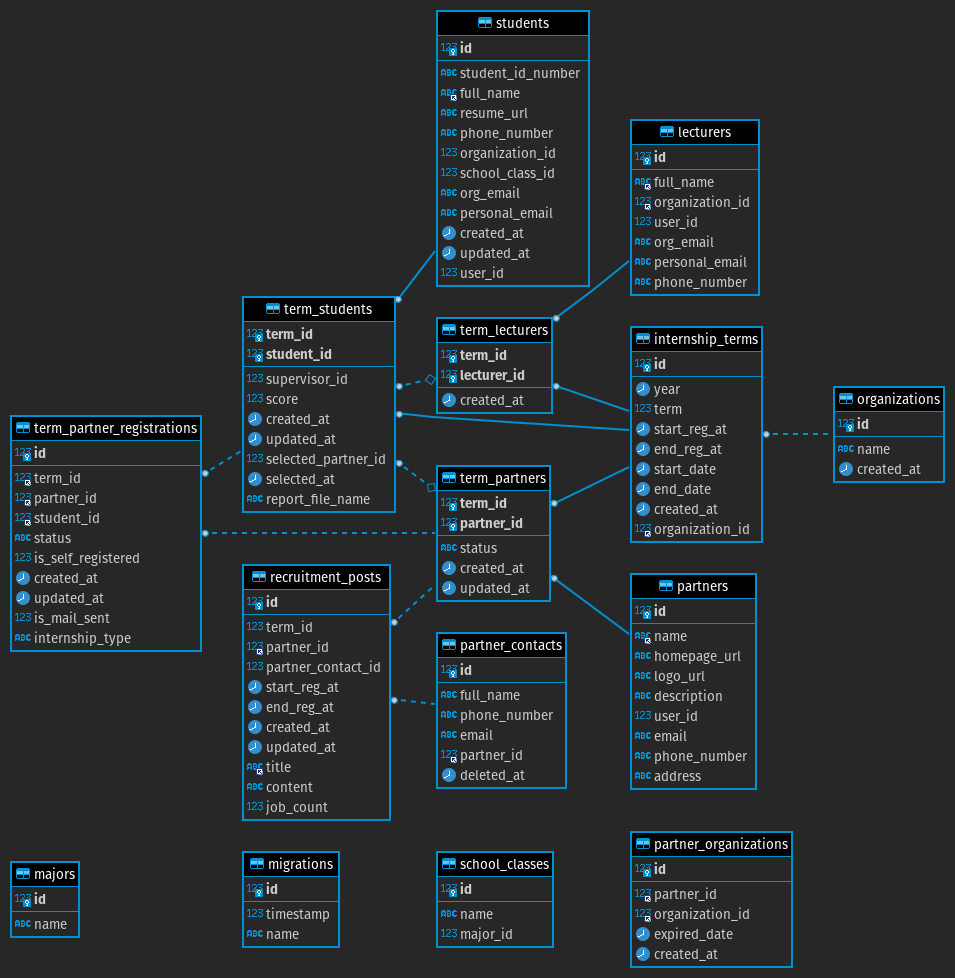
\includegraphics[width=6.5in,height=3.65278in]{vertopal_840b8d8141ff4800a3d2d1a844259cf5/media/image1.png}

Tại trang \emph{Thêm bài đăng}, đối tác có thể tạo bài đăng rồi đăng lên
hệ thống để tuyển dụng sinh viên thực tập.

\subsubsection{Màn hình của Quản trị viên Khoa}

% 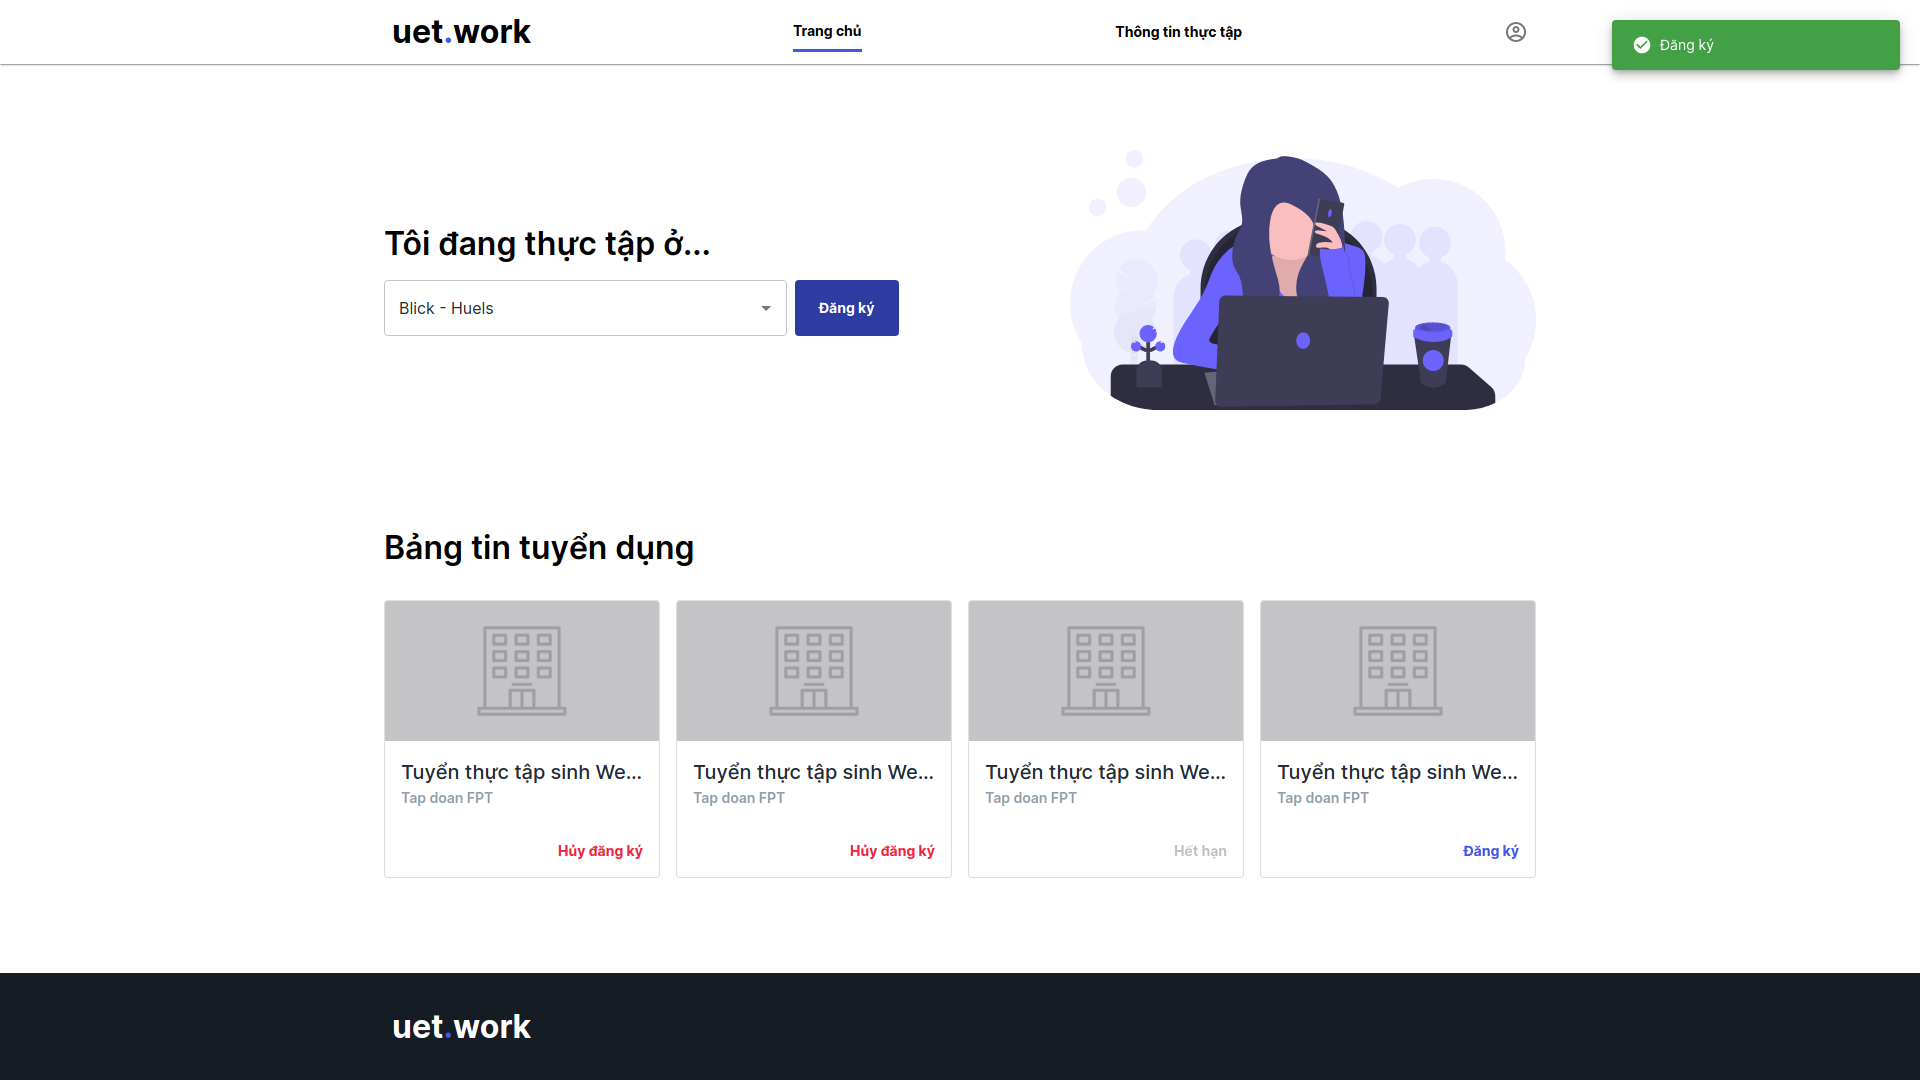
\includegraphics[width=6.5in,height=3.31944in]{vertopal_840b8d8141ff4800a3d2d1a844259cf5/media/image15.png}

Nếu người dùng là \textbf{quản trị viên Khoa}, hệ thống sẽ hiển thị màn
hình trang chủ của quản trị viên Khoa. Tại danh mục \emph{Kỳ thực tập,}
quản trị viên Khoa có thể thực hiện các thao tác quản lý \emph{Danh sách
kỳ thực tập, Bài đăng, Yêu cầu thực tập, Sinh viên, Đơn vị thực tập,
Giảng viên theo kỳ thực tập.}

% 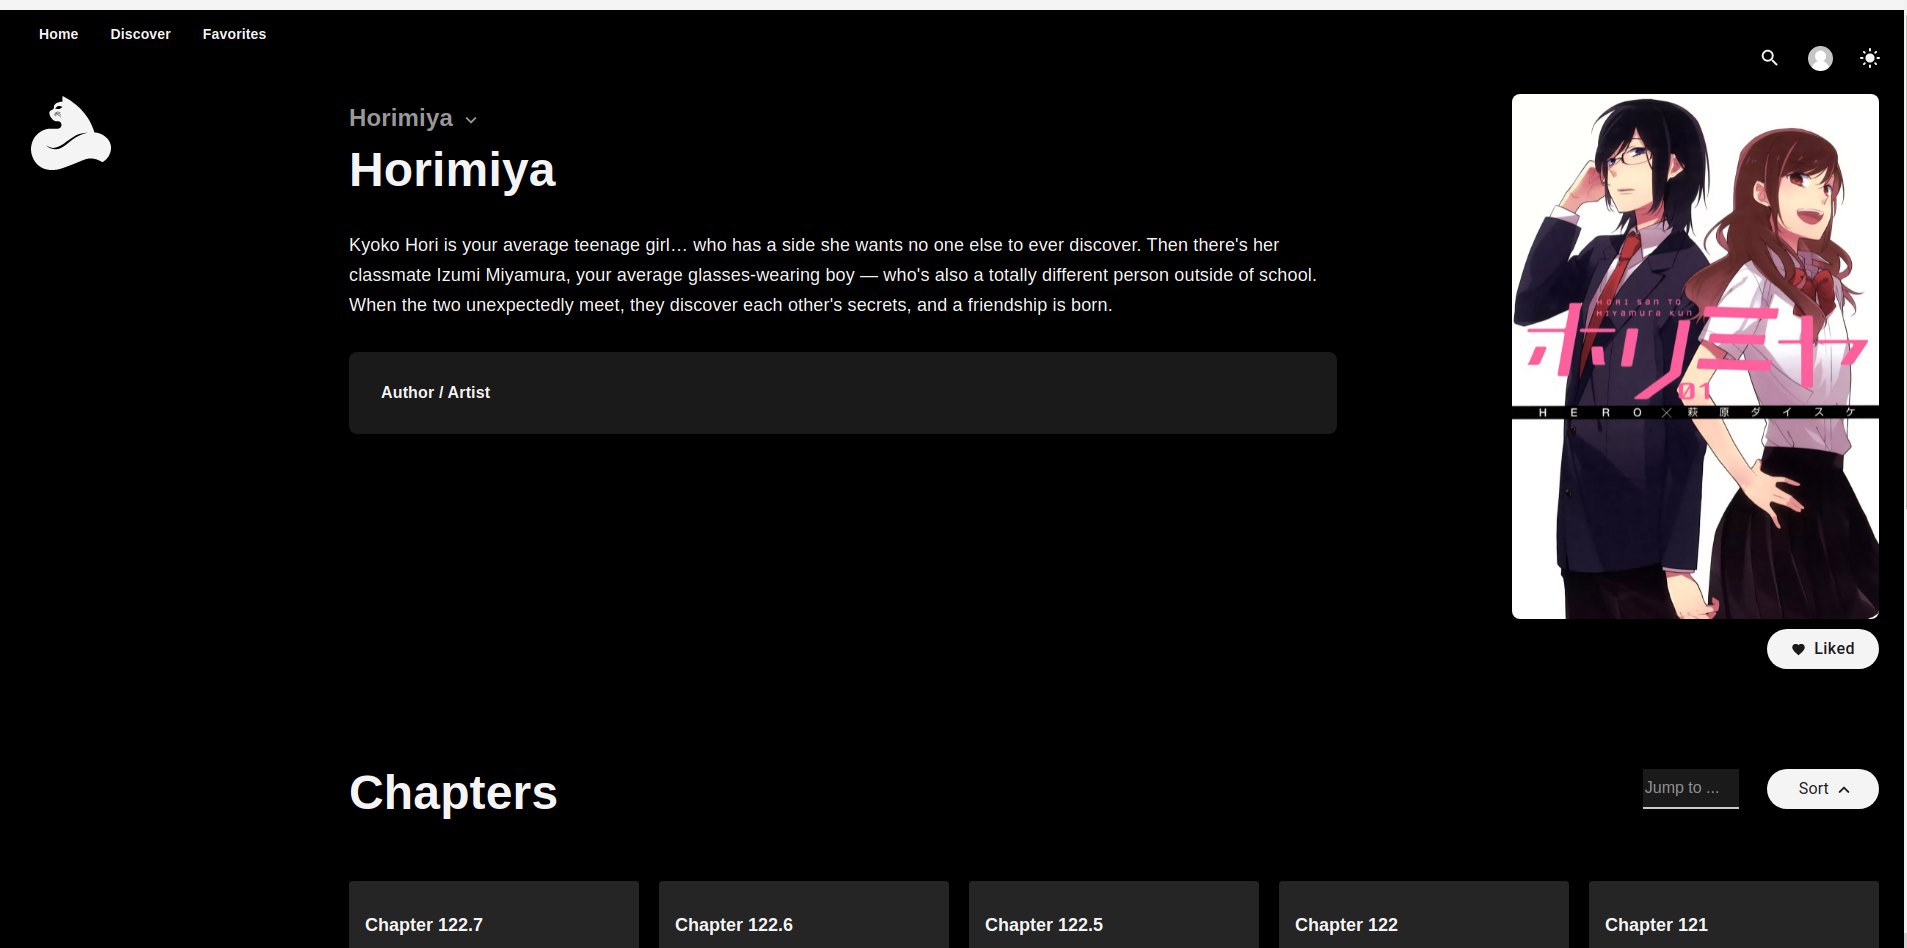
\includegraphics[width=6.5in,height=3.31944in]{vertopal_840b8d8141ff4800a3d2d1a844259cf5/media/image2.png}

Tại danh mục \emph{Người dùng,} quản trị viên Khoa có thể thực hiện các
thao tác quản lý thông tin cá nhân của danh sách \emph{Sinh viên, Đơn vị
thực tập, Giảng viên} tại Khoa của mình.

\end{document}